%%%%%%%%%%%%%%%%%%%%%%%%%%%%%%%%%%%%%%%%%%%%%%%%%%%%%%%%%%%%%%%%%%%%%%%%%%
%  hw1.Rnw
%   
%  Autor: Alexandro Mayoral <https://github.com/bluepill5>  
% 
%%%%%%%%%%%%%%%%%%%%%%%%%%%%%%%%%%%%%%%%%%%%%%%%%%%%%%%%%%%%%%%%%%%%%%%%%%

\documentclass[a4paper]{scrartcl}\usepackage[]{graphicx}\usepackage[]{color}
%% maxwidth is the original width if it is less than linewidth
%% otherwise use linewidth (to make sure the graphics do not exceed the margin)
\makeatletter
\def\maxwidth{ %
  \ifdim\Gin@nat@width>\linewidth
    \linewidth
  \else
    \Gin@nat@width
  \fi
}
\makeatother

\definecolor{fgcolor}{rgb}{0.345, 0.345, 0.345}
\newcommand{\hlnum}[1]{\textcolor[rgb]{0.686,0.059,0.569}{#1}}%
\newcommand{\hlstr}[1]{\textcolor[rgb]{0.192,0.494,0.8}{#1}}%
\newcommand{\hlcom}[1]{\textcolor[rgb]{0.678,0.584,0.686}{\textit{#1}}}%
\newcommand{\hlopt}[1]{\textcolor[rgb]{0,0,0}{#1}}%
\newcommand{\hlstd}[1]{\textcolor[rgb]{0.345,0.345,0.345}{#1}}%
\newcommand{\hlkwa}[1]{\textcolor[rgb]{0.161,0.373,0.58}{\textbf{#1}}}%
\newcommand{\hlkwb}[1]{\textcolor[rgb]{0.69,0.353,0.396}{#1}}%
\newcommand{\hlkwc}[1]{\textcolor[rgb]{0.333,0.667,0.333}{#1}}%
\newcommand{\hlkwd}[1]{\textcolor[rgb]{0.737,0.353,0.396}{\textbf{#1}}}%

\usepackage{framed}
\makeatletter
\newenvironment{kframe}{%
 \def\at@end@of@kframe{}%
 \ifinner\ifhmode%
  \def\at@end@of@kframe{\end{minipage}}%
  \begin{minipage}{\columnwidth}%
 \fi\fi%
 \def\FrameCommand##1{\hskip\@totalleftmargin \hskip-\fboxsep
 \colorbox{shadecolor}{##1}\hskip-\fboxsep
     % There is no \\@totalrightmargin, so:
     \hskip-\linewidth \hskip-\@totalleftmargin \hskip\columnwidth}%
 \MakeFramed {\advance\hsize-\width
   \@totalleftmargin\z@ \linewidth\hsize
   \@setminipage}}%
 {\par\unskip\endMakeFramed%
 \at@end@of@kframe}
\makeatother

\definecolor{shadecolor}{rgb}{.97, .97, .97}
\definecolor{messagecolor}{rgb}{0, 0, 0}
\definecolor{warningcolor}{rgb}{1, 0, 1}
\definecolor{errorcolor}{rgb}{1, 0, 0}
\newenvironment{knitrout}{}{} % an empty environment to be redefined in TeX

\usepackage{alltt}

% Librerías necesarias
\usepackage[utf8]{inputenc}
\usepackage{amsmath}
\usepackage{amsfonts}
\usepackage{amssymb}
\usepackage{enumerate}
\usepackage{fullpage} % Maximiza el uso del espacio en la hoja.
\usepackage[left=2cm,right=2cm,top=2cm,bottom=2cm]{geometry}
\usepackage{dcolumn}
\usepackage{rotating}
\usepackage{float}
\usepackage[section]{placeins}
\usepackage{needspace}
\usepackage{hyperref}
\usepackage{setspace}
\usepackage{pifont}
\usepackage{adjustbox}
\usepackage[table,xcdraw]{xcolor}
\usepackage{graphics}
\onehalfspacing

\author{Alexandro Mayoral, Daniela Chávez y Gerardo Vazquez}
\title{Tarea 1 Análisis y Diseño de Experimentos}
\date{15/03/2015}
\IfFileExists{upquote.sty}{\usepackage{upquote}}{}
\begin{document}
\maketitle




\textbf{Problema 1}
Considere una variable aleatoria $X \sim N(0.5, 1)$ determine la probabilidad de que $X>1$. Elabore la gráfica correspondiente.

\begin{knitrout}
\definecolor{shadecolor}{rgb}{0.969, 0.969, 0.969}\color{fgcolor}\begin{kframe}
\begin{alltt}
\hlcom{# Obtenemos la probailidad de que X > 1}
\hlkwd{pnorm}\hlstd{(}\hlnum{1}\hlstd{,} \hlkwc{mean} \hlstd{=} \hlnum{0.5}\hlstd{,} \hlkwc{sd} \hlstd{=} \hlkwd{sqrt}\hlstd{(}\hlnum{1}\hlstd{),} \hlkwc{lower.tail} \hlstd{= F)}
\end{alltt}
\begin{verbatim}
## [1] 0.3085
\end{verbatim}
\end{kframe}
\end{knitrout}

\noindent A continuación observamos la gráfica:\\

\begin{knitrout}
\definecolor{shadecolor}{rgb}{0.969, 0.969, 0.969}\color{fgcolor}

{\centering 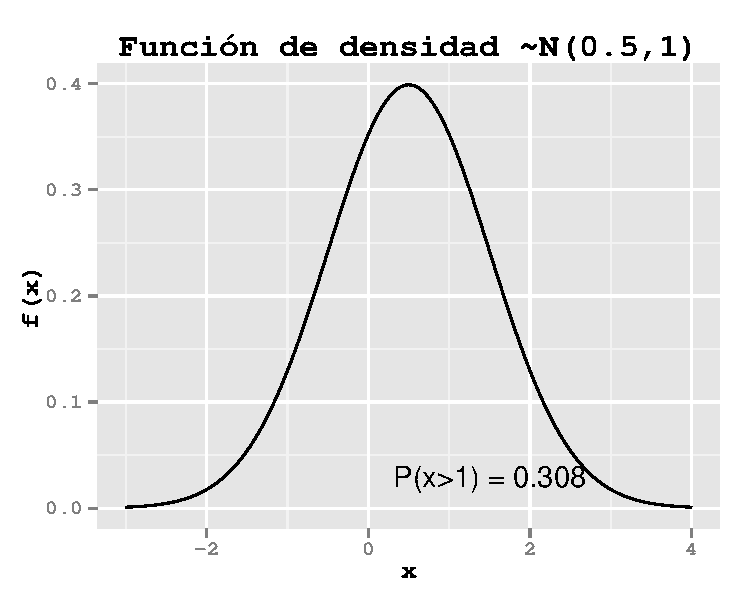
\includegraphics[width=\maxwidth]{figure/unnamed-chunk-3} 

}



\end{knitrout}

\newpage
\textbf{Problema 2}
Se utilizan dos máquinas para llenar botellas de plástico con un volumen neto de 16 onzas. El proceso de llenado se puede suponer normal. Los ingenieros del departamento de calidad sospechan que las dos máquinas llenan a diferente volumen, por lo que se realizó un experimento tomando una muestra al azar de 10 botellas llenadas por cada una de las dos máquinas.

\begin{table}[h!]
\centering
\begin{tabular}[t]{|c|c|c|c|}
\hline
\multicolumn{2}{|c|}{\textbf{máquina 1}}&\multicolumn{2}{|c|}{\textbf{máquina 2}}\\
\hline
16.03&16.01&16.02&16.03\\
16.04&15.96&15.97&16.04\\
16.05&15.98&15.96&16.02\\
16.05&16.02&16.01&16.01\\
16.02&15.99&15.99&16.00\\
\hline
\end{tabular}
\end{table}

\begin{enumerate}[a)]
  \item Pruebe la hipótesis de que el promedio de llenado de las dos máquinas es el mismo vs. es diferente.  Use $\alpha=0.05$. Primero suponiendo que las varianzas son homogéneas y después suponiendo que no son homogéneas.
  \item Calcule un intervalo del 95\% de confianza para la diferencia de las  medias de volumen de llenado de las máquinas.
\end{enumerate}

\noindent Veamos un boxplot de los datos por máquina:

\begin{knitrout}
\definecolor{shadecolor}{rgb}{0.969, 0.969, 0.969}\color{fgcolor}

{\centering 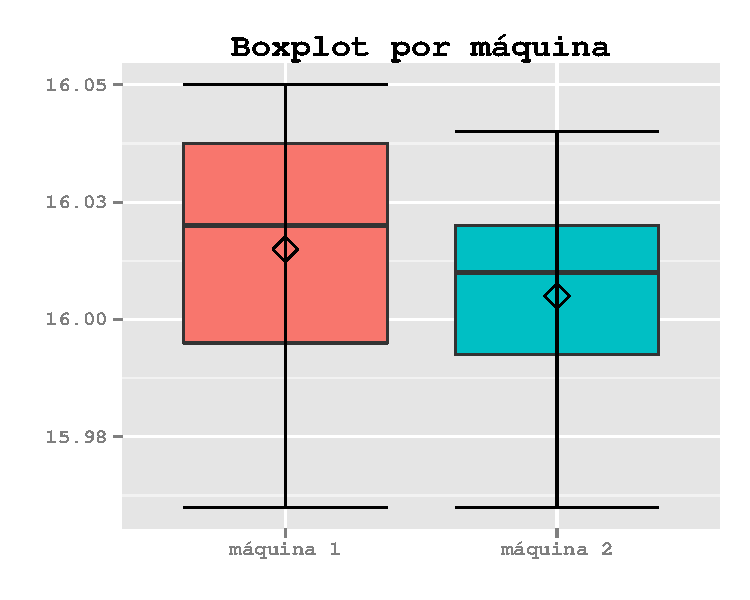
\includegraphics[width=\maxwidth]{figure/unnamed-chunk-4} 

}



\end{knitrout}

\begin{knitrout}
\definecolor{shadecolor}{rgb}{0.969, 0.969, 0.969}\color{fgcolor}\begin{kframe}
\begin{alltt}
\hlcom{# Pruebe la hipótesis de que el promedio de llenado de las dos máquinas }
\hlcom{# es el mismo vs. es diferente}
\hlcom{# Bajo el supuesto de varianzas iguales:}
\hlcom{# Método largo}
\hlcom{# Manipulamos los datos para los cálculos}
\hlstd{datos} \hlkwb{<-} \hlkwd{data.frame}\hlstd{(}\hlkwc{maquina1}\hlstd{=}\hlkwd{subset}\hlstd{(datos, trat} \hlopt{==} \hlstr{"máquina 1"}\hlstd{)[,} \hlstr{"vol"}\hlstd{],}
                    \hlkwc{maquina2}\hlstd{=}\hlkwd{subset}\hlstd{(datos, trat} \hlopt{==} \hlstr{"máquina 2"}\hlstd{)[,} \hlstr{"vol"}\hlstd{])}
\hlcom{# Cálculo de las medias}
\hlkwd{colMeans}\hlstd{(datos)}
\end{alltt}
\begin{verbatim}
## maquina1 maquina2 
##    16.02    16.00
\end{verbatim}
\begin{alltt}
\hlcom{# Cálculo de la diferencia de medias}
\hlstd{dif} \hlkwb{<-} \hlkwd{as.numeric}\hlstd{(}\hlkwd{colMeans}\hlstd{(datos)[}\hlnum{1}\hlstd{]} \hlopt{-} \hlkwd{colMeans}\hlstd{(datos)[}\hlnum{2}\hlstd{])}
\hlstd{S2_1} \hlkwb{<-} \hlkwd{var}\hlstd{(datos[,} \hlnum{1}\hlstd{])}
\hlstd{S2_2} \hlkwb{<-} \hlkwd{var}\hlstd{(datos[,} \hlnum{2}\hlstd{])}
\hlstd{S2_p} \hlkwb{<-} \hlstd{((n1} \hlopt{-} \hlnum{1}\hlstd{)} \hlopt{*} \hlstd{S2_1} \hlopt{+} \hlstd{(n2} \hlopt{-} \hlnum{1}\hlstd{)} \hlopt{*} \hlstd{S2_2)} \hlopt{/} \hlstd{(n1} \hlopt{+} \hlstd{n2} \hlopt{-} \hlnum{2}\hlstd{)}

\hlstd{t_0} \hlkwb{<-} \hlstd{dif}\hlopt{/}\hlstd{(}\hlkwd{sqrt}\hlstd{(S2_p}\hlopt{*}\hlstd{(}\hlnum{1}\hlopt{/}\hlstd{n1} \hlopt{+} \hlnum{1}\hlopt{/}\hlstd{n2))); t_0}
\end{alltt}
\begin{verbatim}
## [1] 0.7989
\end{verbatim}
\begin{alltt}
\hlcom{# Región de rechazo}
\hlstd{alpha} \hlkwb{<-} \hlnum{0.05}
\hlstd{gl} \hlkwb{<-} \hlstd{n1} \hlopt{+} \hlstd{n2} \hlopt{-} \hlnum{2}
\hlstd{t} \hlkwb{<-} \hlkwd{qt}\hlstd{(}\hlnum{1} \hlopt{-} \hlstd{(alpha}\hlopt{/}\hlnum{2}\hlstd{), gl)}
\hlcom{# P-value de 2 colas}
\hlkwd{pt}\hlstd{(t_0, gl,} \hlkwc{lower.tail} \hlstd{=} \hlnum{FALSE}\hlstd{)} \hlopt{*} \hlnum{2}
\end{alltt}
\begin{verbatim}
## [1] 0.4347
\end{verbatim}
\begin{alltt}
\hlcom{# Método corto}
\hlkwd{t.test}\hlstd{(datos[,} \hlnum{1}\hlstd{], datos[,} \hlnum{2}\hlstd{])}
\end{alltt}
\begin{verbatim}
## 
## 	Welch Two Sample t-test
## 
## data:  x and datos[, 2]
## t = 0.7989, df = 17.49, p-value = 0.435
## alternative hypothesis: true difference in means is not equal to 0
## 95 percent confidence interval:
##  -0.01635  0.03635
## sample estimates:
## mean of x mean of y 
##     16.02     16.00
\end{verbatim}
\end{kframe}
\end{knitrout}

\noindent Por lo que bajo la hipótesis $H_0: \mu_1 = \mu_2 (t= 0.7989,p>0.05)$ y asumiendo varianzas iguales, no existe evidencia significativa para rechazar que el promedio del llenado de botellas de la máquina 1 y 2 son iguales. Ahora veamos el caso cuando no consideramos que las varianzas son homogéneas.

\newpage

\begin{knitrout}
\definecolor{shadecolor}{rgb}{0.969, 0.969, 0.969}\color{fgcolor}\begin{kframe}
\begin{alltt}
\hlcom{# Bajo el supuesto de varianzas diferentes:}
\hlcom{# Método largo}
\hlcom{# t welch}
\hlstd{tw} \hlkwb{<-} \hlstd{dif} \hlopt{/} \hlstd{(}\hlkwd{sqrt}\hlstd{(S2_1}\hlopt{/}\hlstd{n1} \hlopt{+} \hlstd{S2_2}\hlopt{/}\hlstd{n2)); tw}
\end{alltt}
\begin{verbatim}
## [1] 0.7989
\end{verbatim}
\begin{alltt}
\hlcom{#región de rechazo}
\hlstd{gl_tw} \hlkwb{<-} \hlstd{(S2_1}\hlopt{/}\hlstd{n1} \hlopt{+} \hlstd{S2_2}\hlopt{/}\hlstd{n2)}\hlopt{**}\hlnum{2} \hlopt{/} \hlstd{(((S2_1}\hlopt{/}\hlstd{n1)}\hlopt{**}\hlnum{2}\hlopt{/}\hlstd{(n1} \hlopt{-} \hlnum{1}\hlstd{))} \hlopt{+} \hlstd{((S2_2}\hlopt{/}\hlstd{n2)}\hlopt{**}\hlnum{2}\hlopt{/}\hlstd{(n2}\hlopt{-}\hlnum{1}\hlstd{)))}
\hlstd{t2} \hlkwb{<-} \hlkwd{qt}\hlstd{(}\hlnum{1}\hlopt{-}\hlstd{(alpha}\hlopt{/}\hlnum{2}\hlstd{), gl_tw); t2}
\end{alltt}
\begin{verbatim}
## [1] 2.105
\end{verbatim}
\begin{alltt}
\hlcom{# P-value}
\hlkwd{pt}\hlstd{(tw, gl_tw,} \hlkwc{lower.tail} \hlstd{=} \hlnum{FALSE}\hlstd{)} \hlopt{*} \hlnum{2}
\end{alltt}
\begin{verbatim}
## [1] 0.435
\end{verbatim}
\begin{alltt}
\hlcom{# Método Corto}
\hlkwd{t.test}\hlstd{(datos[,} \hlnum{1}\hlstd{], datos[,} \hlnum{2}\hlstd{],} \hlkwc{var.equal}\hlstd{=F)}
\end{alltt}
\begin{verbatim}
## 
## 	Welch Two Sample t-test
## 
## data:  x and datos[, 2]
## t = 0.7989, df = 17.49, p-value = 0.435
## alternative hypothesis: true difference in means is not equal to 0
## 95 percent confidence interval:
##  -0.01635  0.03635
## sample estimates:
## mean of x mean of y 
##     16.02     16.00
\end{verbatim}
\end{kframe}
\end{knitrout}

\noindent Por lo qué observamos que tampoco existe evidencia para rechazar la hipótesis nula ($H_0: \mu_1 = \mu_2 (t= 0.7989,p>0.05)$), asumiendo que se tienen varianzas distintas. A continuación mostramos la prueba F para evaluar la exitencia de homocedasticidad

\begin{knitrout}
\definecolor{shadecolor}{rgb}{0.969, 0.969, 0.969}\color{fgcolor}\begin{kframe}
\begin{alltt}
\hlkwd{var.test}\hlstd{(datos[,} \hlnum{1}\hlstd{], datos[,} \hlnum{2}\hlstd{])}
\end{alltt}
\begin{verbatim}
## 
## 	F test to compare two variances
## 
## data:  datos[, 1] and datos[, 2]
## F = 1.41, num df = 9, denom df = 9, p-value = 0.6168
## alternative hypothesis: true ratio of variances is not equal to 1
## 95 percent confidence interval:
##  0.3503 5.6777
## sample estimates:
## ratio of variances 
##               1.41
\end{verbatim}
\end{kframe}
\end{knitrout}

\noindent Por lo que no hay evidencia para rechazar la hipótesis de homocedasticidad a un nivel de significancia del $0.05$.\\

\noindent Ahora calculamos los intervalos del $95\%$ de confianza para la diferencia de medias:

\begin{knitrout}
\definecolor{shadecolor}{rgb}{0.969, 0.969, 0.969}\color{fgcolor}\begin{kframe}
\begin{alltt}
\hlcom{# Bajo el supuesto de homocedasticidad}
\hlstd{ic_vi} \hlkwb{<-} \hlkwd{cbind}\hlstd{(dif} \hlopt{-} \hlstd{t} \hlopt{*} \hlkwd{sqrt}\hlstd{(S2_p}\hlopt{*}\hlstd{(}\hlnum{1}\hlopt{/}\hlstd{n1} \hlopt{+} \hlnum{1}\hlopt{/}\hlstd{n2)),}
               \hlstd{dif} \hlopt{+} \hlstd{t} \hlopt{*} \hlkwd{sqrt}\hlstd{(S2_p}\hlopt{*}\hlstd{(}\hlnum{1}\hlopt{/}\hlstd{n1} \hlopt{+} \hlnum{1}\hlopt{/}\hlstd{n2)))}
\hlkwd{colnames}\hlstd{(ic_vi)} \hlkwb{<-} \hlkwd{cbind}\hlstd{(}\hlstr{"límite inferior"}\hlstd{,}\hlstr{"límite superior"}\hlstd{);ic_vi}
\end{alltt}
\begin{verbatim}
##      límite inferior límite superior
## [1,]         -0.0163          0.0363
\end{verbatim}
\begin{alltt}
\hlcom{# Amplitud del intervalo}
\hlkwd{diff}\hlstd{(}\hlkwd{as.vector}\hlstd{(ic_vi))}
\end{alltt}
\begin{verbatim}
## [1] 0.05259
\end{verbatim}
\begin{alltt}
\hlcom{# Bajo el supuesto de no homocedasticidad}
\hlstd{ic_vd} \hlkwb{<-} \hlkwd{cbind}\hlstd{(dif} \hlopt{-} \hlstd{t2} \hlopt{*} \hlkwd{sqrt}\hlstd{(S2_1}\hlopt{/}\hlstd{n1} \hlopt{+} \hlstd{S2_2}\hlopt{/}\hlstd{n2),}
               \hlstd{dif} \hlopt{+} \hlstd{t2} \hlopt{*} \hlkwd{sqrt}\hlstd{(S2_1}\hlopt{/}\hlstd{n1} \hlopt{+} \hlstd{S2_2}\hlopt{/}\hlstd{n2))}
\hlkwd{colnames}\hlstd{(ic_vd)} \hlkwb{<-} \hlkwd{cbind}\hlstd{(}\hlstr{"límite inferior"}\hlstd{,}\hlstr{"límite superior"}\hlstd{);ic_vd}
\end{alltt}
\begin{verbatim}
##      límite inferior límite superior
## [1,]        -0.01635         0.03635
\end{verbatim}
\begin{alltt}
\hlcom{# Amplitud del intervalo}
\hlkwd{diff}\hlstd{(}\hlkwd{as.vector}\hlstd{(ic_vd))}
\end{alltt}
\begin{verbatim}
## [1] 0.0527
\end{verbatim}
\end{kframe}
\end{knitrout}

\noindent Por lo anterior vemos que el intervalo bajo el supuesto de homocedasticidad es más pequeño, además ambos intervalos contienen al cero, por lo que tenemos una confianza del $95\%$ de que no existe diferencia en el promedio de llenado de botellas en ambas máquinas. Es importante también mencionar que uno de los puestos que se usó al realizar los contrastes de hipótesis fue el de normalidad de los datos, por lo qué se debería aplicar una prueba para evaluar este supuesto.

\newpage
\textbf{Problema 3}
Considere un diseño de experimento unifactorial (efectos fijos) de 4 tratamientos donde se tienen un total de 24 unidades experimentales y conteste lo siguiente:

\begin{itemize}
  \item Complete la siguiente tabla ANOVA:
\end{itemize}

\begin{table}[h]
\centering
\begin{adjustbox}{max width=\textwidth}
\begin{tabular}{|l|c|ccc}
\hline
\rowcolor[HTML]{C0C0C0} 
\textbf{FV} & \multicolumn{1}{l|}{\cellcolor[HTML]{C0C0C0}\textbf{g.l.}} & \multicolumn{1}{l|}{\cellcolor[HTML]{C0C0C0}\textbf{S.C.}} & \multicolumn{1}{l|}{\cellcolor[HTML]{C0C0C0}\textbf{C.M.}} & \multicolumn{1}{l|}{\cellcolor[HTML]{C0C0C0}\textbf{F}} \\ \hline
\cellcolor[HTML]{C0C0C0}\textbf{Modelo} &  & \multicolumn{1}{c|}{} & \multicolumn{1}{c|}{} & \multicolumn{1}{c|}{0.5655} \\ \hline
\cellcolor[HTML]{C0C0C0}\textbf{Error} &  & \multicolumn{1}{c|}{} & \multicolumn{1}{c|}{16.02} &  \\ \cline{1-4}
\cellcolor[HTML]{C0C0C0}\textbf{Total} &  &  &  &  \\ \cline{1-2}
\end{tabular}
\end{adjustbox}
\end{table}

\noindent La tabla la podemos completar de la siguiente forma:\\

\begin{table}[h]
\centering
\begin{adjustbox}{max width=\textwidth}
\begin{tabular}{|l|c|c|cc}
\hline
\rowcolor[HTML]{C0C0C0} 
\textbf{FV} & \textbf{g.l.} & \textbf{S.C.} & \multicolumn{1}{c|}{\cellcolor[HTML]{C0C0C0}\textbf{C.M.}} & \multicolumn{1}{c|}{\cellcolor[HTML]{C0C0C0}\textbf{F}} \\ \hline
\cellcolor[HTML]{C0C0C0}\textbf{Modelo} & t - 1 = 4 - 1 = 3 & SSt = CMt * (t - 1) = 27.178 & \multicolumn{1}{c|}{CMt = F * CME = 9.059} & \multicolumn{1}{c|}{F = CMt / CME = 0.5655} \\ \hline
\cellcolor[HTML]{C0C0C0}\textbf{Error} & n - t = 96 - 4 = 92 & SSE = CME * (n - t) = 16.02 * 92 = 1473.84 & \multicolumn{1}{c|}{CME = 16.02} &  \\ \cline{1-4}
\cellcolor[HTML]{C0C0C0}\textbf{Total} & n - 1 = 96 -1 = 95 & SStotal = SSt + SSE &  &  \\ \cline{1-3}
\end{tabular}
\end{adjustbox}
\end{table}

\begin{itemize}
  \item Determine el valor $\hat{\sigma^2}$
\end{itemize}
De la tabla sabemos que $CME = \hat{\sigma^2} = 16.02$

\begin{itemize}
  \item Con $\alpha = 0.05$ se rechaza o no la hipótesis de igualdad de medias?
\end{itemize}
\begin{knitrout}
\definecolor{shadecolor}{rgb}{0.969, 0.969, 0.969}\color{fgcolor}\begin{kframe}
\begin{alltt}
\hlstd{alpha} \hlkwb{<-} \hlnum{0.05}
\hlkwd{qf}\hlstd{(}\hlnum{1} \hlopt{-} \hlstd{alpha,} \hlkwc{df1}\hlstd{=} \hlnum{3}\hlstd{,} \hlkwc{df2} \hlstd{=} \hlnum{92}\hlstd{)}
\end{alltt}
\begin{verbatim}
## [1] 2.704
\end{verbatim}
\end{kframe}
\end{knitrout}
Entonces sabemo que valores grandes de $F$ llevan a rechazar la hipótesis de nula de igualdad de medias, pero como $F = 0.5655 < F_{t-1, n-t}^{0.05} = 2.704)$ no tenemos evidencia para rechzar la hipótesis nula a una significancia del $5\%$.


\begin{itemize}
  \item Con $\alpha = 0.01$ se rechaza o no la hipótesis de igualdad de medias?
\end{itemize}
\begin{knitrout}
\definecolor{shadecolor}{rgb}{0.969, 0.969, 0.969}\color{fgcolor}\begin{kframe}
\begin{alltt}
\hlstd{alpha} \hlkwb{<-} \hlnum{0.01}
\hlkwd{qf}\hlstd{(}\hlnum{1} \hlopt{-} \hlstd{alpha,} \hlkwc{df1}\hlstd{=} \hlnum{3}\hlstd{,} \hlkwc{df2} \hlstd{=} \hlnum{92}\hlstd{)}
\end{alltt}
\begin{verbatim}
## [1] 4.002
\end{verbatim}
\end{kframe}
\end{knitrout}
En este caso $F = 0.5655 < F_{t-1, n-t}^{0.05} = 4.002)$ por lo que tampoco tenemos evidencia para rechazar la hipótesis nula a una significancia del $5\%$.

\newpage
\textbf{Problema 4}
En un diseño de experimetos unifactorial de efectos fijos completamente al azar, se tiene 5 tratamientos con 5 repeticiones cada uno. El estadístico de prueba $F_0$ es igual a 3.5. Elabore la gráfica que muestre las regiones de rechazo con $\alpha = 0.05$ y con $\alpha = 0.01$; ubique la posición del estadístico $F_0$, analice y concluya si existe evidencia para determinar la igualdad de medias de los tratamientos (tanto para $\alpha = 0.05$ como para $\alpha = 0.01$).\\

Como tenemos 5 tratamientos y 5 repeticiones entonces tenemos que: $t = 5$, $r = 5$ y $n = 25$. Por lo que tenemos que obtener $F_{t-1, n-t}^{1 - \alpha}$, es decir, $F_{4, 20}^{0.95}$ y $F_{4, 20}^{0.99}$, donde $H_0: \mu_1 = \mu_2 ... =\mu_5$, para comparar con nuestro estadístico de prueba: 

\begin{knitrout}
\definecolor{shadecolor}{rgb}{0.969, 0.969, 0.969}\color{fgcolor}\begin{kframe}
\begin{alltt}
\hlcom{# Significancia del 5%}
\hlstd{F95} \hlkwb{<-} \hlkwd{qf}\hlstd{(}\hlnum{0.95}\hlstd{,} \hlkwc{df1} \hlstd{=} \hlnum{4}\hlstd{,} \hlkwc{df2} \hlstd{=} \hlnum{20}\hlstd{); F95}
\end{alltt}
\begin{verbatim}
## [1] 2.866
\end{verbatim}
\begin{alltt}
\hlcom{# Significancia del 1%}
\hlstd{F99} \hlkwb{<-} \hlkwd{qf}\hlstd{(}\hlnum{0.99}\hlstd{,} \hlkwc{df1} \hlstd{=} \hlnum{4}\hlstd{,} \hlkwc{df2} \hlstd{=} \hlnum{20}\hlstd{); F99}
\end{alltt}
\begin{verbatim}
## [1] 4.431
\end{verbatim}
\end{kframe}
\end{knitrout}

\begin{knitrout}
\definecolor{shadecolor}{rgb}{0.969, 0.969, 0.969}\color{fgcolor}

{\centering 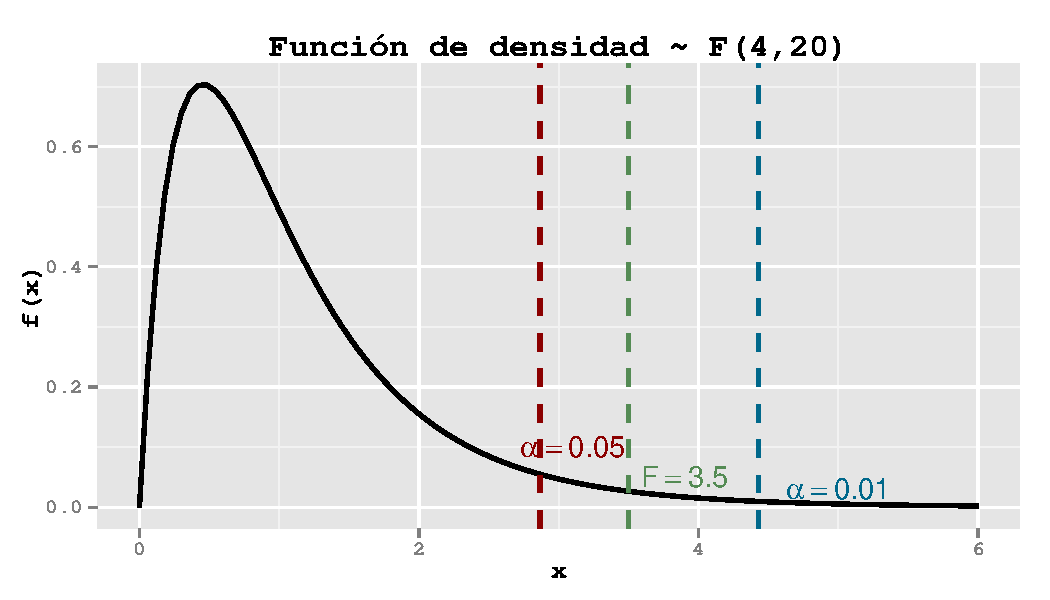
\includegraphics[width=\maxwidth]{figure/unnamed-chunk-12} 

}



\end{knitrout}

\noindent Por lo que para una significancia del $95\%$ tenemos evidencia para rechazar la hipótesis nula de igualdad de medias ($F_0 = 3.5 >  F_{4,20}^{0.05} = 2.866$), mientras que para una significancia del $99\%$ no tenemos evidencia para rechazar la hipótesis nula de igualdad de medias ($F_0 = 3.5 <  F_{4,20}^{0.01} = 4.431$).


\newpage
\textbf{Problema 5}
Los siguiente datos muestran las medidas de hemoglobina (gramos por 100ml) en la sangre de 40 ejemplares de una especie de truchas marrones. Las truchas se haían dividido al azar en cuatro grupos de 10 y cada grupo se había asignado, también al azar, a un criadero de cuatro diferentes. En cada criadero se añadía a la dieta de los peces una cantidad distinta de sulfamerazina por cada cien libras de comida. En concreto: 0, 5, 10 y 15 gramos. Las mediciones de hemoglobina se tomaron después de 35 días.

\begin{table}[h!]
\centering
\begin{tabular}[t]{|c|c|}
\hline
\textbf{Sulfametazina }(g/libras de comida)&\textbf{Hemoglobina en sangre} (g/100 ml)\\ 
\hline
\textbf{0}&6.7,  7.8,  5.5,  8.4,  7.0,  7.8,  8.6,  7.4,  5.8,  7.0\\
\hline
\textbf{5}&9.9,  8.4, 10.4,  9.3,  10.7  ,11.9 , 7.1,  6.4,  8.6,  10.6\\
\hline
\textbf{10}&10.4,  8.1, 10.6 , 8.7,  10.7,  9.1,  8.8 , 8.1,  7.8,  8.0\\
\hline
\textbf{15}&9.9,  9.3 , 7.2 , 7.8 , 9.3,  10.2 , 8.7,  8.6, 9.3,  7.2 \\
\hline
\end{tabular}
\end{table}

Se pide que:

\begin{itemize}
  \item Elabore el modelo de diseño de experimentos correspondiente, haciendo explícitos los elementos que lo componen (variable respuesta, factores, supuestos, unidad experimental, ... etc.)
\end{itemize}

\noindent\emph{Diseño}: Diseño completamente al azar\\
\emph{Variable respuesta}: Concentración de hemoglobina (gramos por 100 ml)\\
\emph{Unidad experimental}: Trucha marrón\\
\emph{Factor(es)}: Concentración de sulfamerazina\\
\emph{Niveles}: 4 niveles de concetración de sulfamerazina (0, 5, 10, 15 g/100 lb comida)\\

\noindent Lo anterior supone homogeneidad en las truchas al igual que las condiciones de cada criadero.

\begin{itemize}
  \item Elabore la gráfica de caja tratamientos-hemoglobina, analícela y determine si existe evidencia visual para determinar la igualdad de medias de los tratamientos.
\end{itemize}

\begin{knitrout}
\definecolor{shadecolor}{rgb}{0.969, 0.969, 0.969}\color{fgcolor}

{\centering 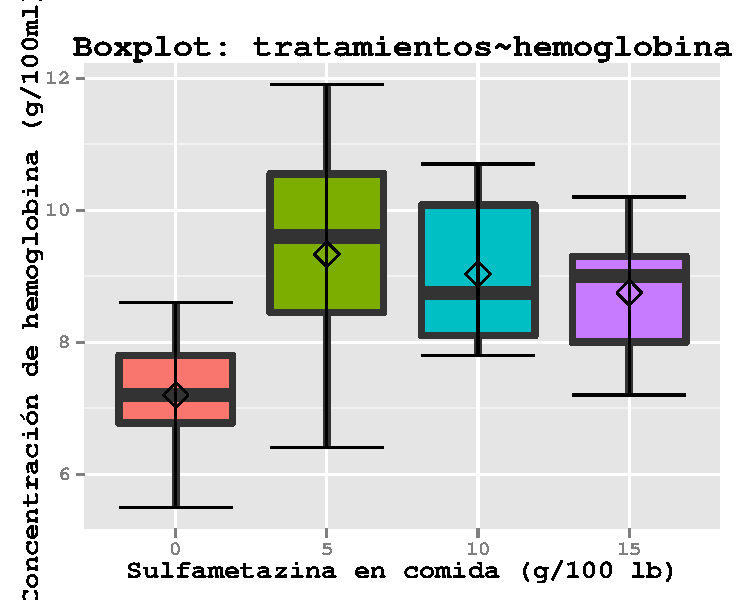
\includegraphics[width=\maxwidth]{figure/unnamed-chunk-13} 

}



\end{knitrout}

\noindent Dada la gráfica anterior podemos observar que la media en la medición de concentración de hemoglobina del grupo control (0 g de sulfametazina) es menor a la de los demás grupos, de los cuales el de 10g y 15g de sulfametazina parecen similares y el de 5g es mayor pero con una varianza mayor al de todos los grupos, por lo que no podemos determinar que hay algún efecto de los tratamientos.

\begin{itemize}
  \item Construya la tabla ANOVA, analícela y concluya ($\alpha = 0.05$)
\end{itemize}
\begin{knitrout}
\definecolor{shadecolor}{rgb}{0.969, 0.969, 0.969}\color{fgcolor}\begin{kframe}
\begin{alltt}
\hlcom{# Creamos un pequeña funciòn para calcular la tabla ANOVA}
\hlstd{myANDEVA} \hlkwb{<-} \hlkwa{function}\hlstd{(}\hlkwc{n}\hlstd{,} \hlkwc{t}\hlstd{,} \hlkwc{data}\hlstd{,} \hlkwc{value}\hlstd{,} \hlkwc{factor}\hlstd{) \{}
    \hlcom{# Crea la tabla de análisis de varianza}
    \hlcom{# n: Tamaño de la muestra}
    \hlcom{# t: Número de tratamientos}
    \hlcom{# data: Data.frame con los datos}
    \hlcom{# value: Variable respuesta}
    \hlcom{# factor: Variable que indica el factor}

    \hlcom{# Calculamos la media general}
    \hlstd{mu} \hlkwb{<-} \hlkwd{mean}\hlstd{(data[, value])}
    \hlcom{# Calculamos la suma de los errores del modelo reducido}
    \hlstd{SSE_r} \hlkwb{<-} \hlkwd{sum}\hlstd{((data[, value]} \hlopt{-} \hlstd{mu)}\hlopt{**}\hlnum{2}\hlstd{)}
    \hlcom{# Ahora calculamos la suma de los errores del modelo completo}
    \hlstd{SSE_c} \hlkwb{<-} \hlkwd{sum}\hlstd{(}
        \hlkwd{unlist}\hlstd{(}
            \hlkwd{lapply}\hlstd{(}
                \hlkwd{split}\hlstd{(data, data[, factor]),}
                \hlkwa{function}\hlstd{(}\hlkwc{x}\hlstd{)} \hlkwd{sum}\hlstd{((x[, value]} \hlopt{-} \hlkwd{mean}\hlstd{(x[, value]))}\hlopt{**}\hlnum{2}\hlstd{))))}
    \hlcom{# Calculamos la suma de los errores por tratamiento}
    \hlstd{SS_t} \hlkwb{<-} \hlstd{SSE_r} \hlopt{-} \hlstd{SSE_c}
    \hlcom{# Calculamos la suma de los errores totales}
    \hlstd{SS_total} \hlkwb{<-} \hlstd{SS_t} \hlopt{+} \hlstd{SSE_c}
    \hlcom{# Calculamos la suma de los errores entre sus grados de libertad}
    \hlstd{CM_t} \hlkwb{<-} \hlstd{SS_t} \hlopt{/} \hlstd{(t} \hlopt{-} \hlnum{1}\hlstd{)}
    \hlstd{CME} \hlkwb{<-} \hlstd{SSE_c} \hlopt{/} \hlstd{(n} \hlopt{-} \hlstd{t)}
    \hlcom{# Claculamos el estadístico de prueba F_0}
    \hlstd{F_0} \hlkwb{<-} \hlstd{CM_t} \hlopt{/} \hlstd{CME}
    \hlcom{# Ahora el p-value}
    \hlstd{p_val} \hlkwb{<-} \hlkwd{pf}\hlstd{(F_0, t} \hlopt{-} \hlnum{1}\hlstd{, n} \hlopt{-} \hlstd{t,} \hlkwc{lower.tail} \hlstd{=} \hlnum{FALSE}\hlstd{)}
    \hlcom{# Ahora creamos la tabla}
    \hlstd{gl} \hlkwb{<-} \hlkwd{c}\hlstd{(t} \hlopt{-} \hlnum{1}\hlstd{, n} \hlopt{-} \hlstd{t, n} \hlopt{-} \hlnum{1}\hlstd{)}
    \hlstd{SS} \hlkwb{<-} \hlkwd{round}\hlstd{(}\hlkwd{c}\hlstd{(SS_t, SSE_c, SS_total),} \hlkwc{digits} \hlstd{=} \hlnum{2}\hlstd{)}
    \hlstd{CM} \hlkwb{<-} \hlkwd{c}\hlstd{(}\hlkwd{round}\hlstd{(CM_t,} \hlkwc{digits} \hlstd{=} \hlnum{2}\hlstd{),} \hlkwd{round}\hlstd{(CME,} \hlkwc{digits} \hlstd{=} \hlnum{2}\hlstd{),} \hlstr{""}\hlstd{)}
    \hlstd{F_value} \hlkwb{<-} \hlkwd{c}\hlstd{(}\hlkwd{round}\hlstd{(F_0,} \hlkwc{digits} \hlstd{=} \hlnum{2}\hlstd{),} \hlstr{""}\hlstd{,} \hlstr{""}\hlstd{)}
    \hlstd{p_value} \hlkwb{<-} \hlkwd{c}\hlstd{(}\hlkwd{round}\hlstd{(p_val,} \hlkwc{digits} \hlstd{=} \hlnum{4}\hlstd{),} \hlstr{""}\hlstd{,} \hlstr{""}\hlstd{)}
    \hlstd{andeva} \hlkwb{<-} \hlkwd{data.frame}\hlstd{(gl, SS, CM, F_value, p_value)}
    \hlcom{# Nombramos a las columnas y renglones}
    \hlkwd{colnames}\hlstd{(andeva)} \hlkwb{<-} \hlkwd{c}\hlstd{(}\hlstr{"g.l."}\hlstd{,} \hlstr{"S.S."}\hlstd{,} \hlstr{"C.M."}\hlstd{,} \hlstr{"F"}\hlstd{,} \hlstr{"p-value"}\hlstd{)}
    \hlkwd{rownames}\hlstd{(andeva)} \hlkwb{<-} \hlkwd{c}\hlstd{(}\hlstr{"Tratamientos"}\hlstd{,} \hlstr{"Error"}\hlstd{,} \hlstr{"Total"}\hlstd{)}
    \hlstd{andeva}
\hlstd{\}}
\hlkwd{myANDEVA}\hlstd{(}\hlkwc{n} \hlstd{=} \hlnum{40}\hlstd{,} \hlkwc{t} \hlstd{=} \hlnum{4}\hlstd{,} \hlkwc{data} \hlstd{= peces,} \hlkwc{value} \hlstd{=} \hlstr{"hemo"}\hlstd{,} \hlkwc{factor} \hlstd{=} \hlstr{"trat"}\hlstd{)}
\end{alltt}
\begin{verbatim}
##              g.l.  S.S. C.M.    F p-value
## Tratamientos    3 26.98 8.99 5.63  0.0029
## Error          36 57.53  1.6             
## Total          39 84.51
\end{verbatim}
\begin{alltt}
\hlcom{# O ajustando el modelo}
\hlstd{pecesMod} \hlkwb{<-} \hlkwd{lm}\hlstd{(hemo} \hlopt{~} \hlstd{trat,} \hlkwc{data} \hlstd{= peces)}
\hlkwd{anova}\hlstd{(pecesMod)}
\end{alltt}
\begin{verbatim}
## Analysis of Variance Table
## 
## Response: hemo
##           Df Sum Sq Mean Sq F value Pr(>F)   
## trat       3   27.0    8.99    5.63 0.0029 **
## Residuals 36   57.5    1.60                  
## ---
## Signif. codes:  0 '***' 0.001 '**' 0.01 '*' 0.05 '.' 0.1 ' ' 1
\end{verbatim}
\end{kframe}
\end{knitrout}

Entonce considerando una significancia del $5\%$ tenemos evidencia para rechazar la hipótesis nula de igualdad de medias, es decir, lo que podemos decir es que el promedio de concentración de hemoglobina difiere en almenos un tratamiento.


\begin{itemize}
  \item Determine qué tratamientos tienen efectos estadísticamente iguales
\end{itemize}

Un forma sería realizar una prueba de diferencia de medias para cada una de los tratamientos pero esto provoca que la significancia global sea mayor a la significancia de cada prueba. Entonces una solución bajo el supuesto de \emph´{homocedasticidad} es usar el critero de Tukey. La idea es establecer un umbral, se calculan todas las diferencias de de medias muestrales entre los t niveles del factor estudiado. Las diferencias que estén por encima de ese umbral se consideran diferencias significativas, las que no lo estén se considerán diferencias no significativas.

\begin{knitrout}
\definecolor{shadecolor}{rgb}{0.969, 0.969, 0.969}\color{fgcolor}\begin{kframe}
\begin{alltt}
\hlcom{# Prueba de Tukey}
\hlstd{tukey} \hlkwb{<-} \hlkwd{TukeyHSD}\hlstd{(}\hlkwd{aov}\hlstd{(pecesMod),} \hlkwc{conf.level} \hlstd{=} \hlnum{0.95}\hlstd{); tukey}
\end{alltt}
\begin{verbatim}
##   Tukey multiple comparisons of means
##     95% family-wise confidence level
## 
## Fit: aov(formula = pecesMod)
## 
## $trat
##        diff      lwr    upr  p adj
## 5-0    2.13  0.60745 3.6526 0.0032
## 10-0   1.83  0.30745 3.3526 0.0132
## 15-0   1.55  0.02745 3.0726 0.0447
## 10-5  -0.30 -1.82255 1.2226 0.9511
## 15-5  -0.58 -2.10255 0.9426 0.7355
## 15-10 -0.28 -1.80255 1.2426 0.9596
\end{verbatim}
\end{kframe}
\end{knitrout}

\noindent Por lo qué lo que observamos diferencias significativas ($\alpha = 0.05$) del grupo control con demás tratamientos y entre los demás tratamientos no observamos una diferencia significativa. Gráficamente podemos ver los intervalos de confianza.

\begin{knitrout}
\definecolor{shadecolor}{rgb}{0.969, 0.969, 0.969}\color{fgcolor}

{\centering 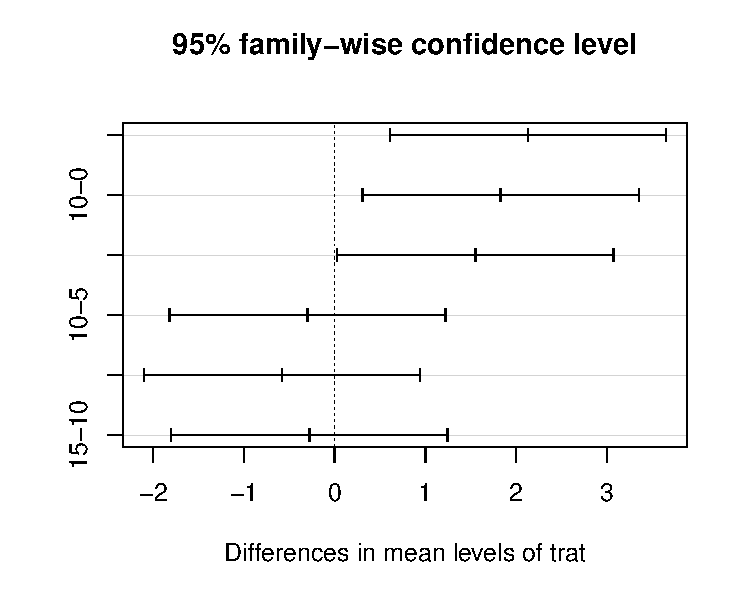
\includegraphics[width=\maxwidth]{figure/unnamed-chunk-16} 

}



\end{knitrout}


\begin{itemize}
  \item Construya las gráficas de los residuos necesarias para verificar los supuestos de homocedasticidad y normalidad. Utilice la prueba de Bartlett para verificar el supuesto de homogeneidad de varianzas 
\end{itemize}

\begin{knitrout}
\definecolor{shadecolor}{rgb}{0.969, 0.969, 0.969}\color{fgcolor}

{\centering 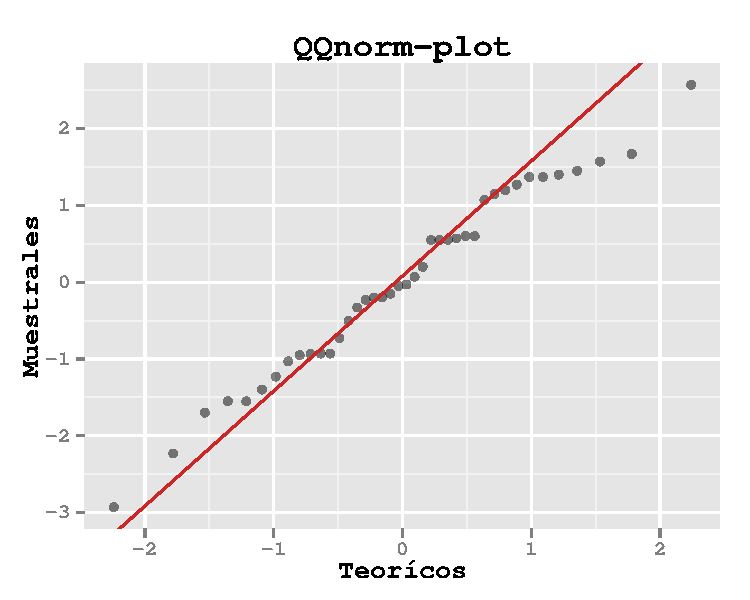
\includegraphics[width=\maxwidth]{figure/unnamed-chunk-171} 

}




{\centering 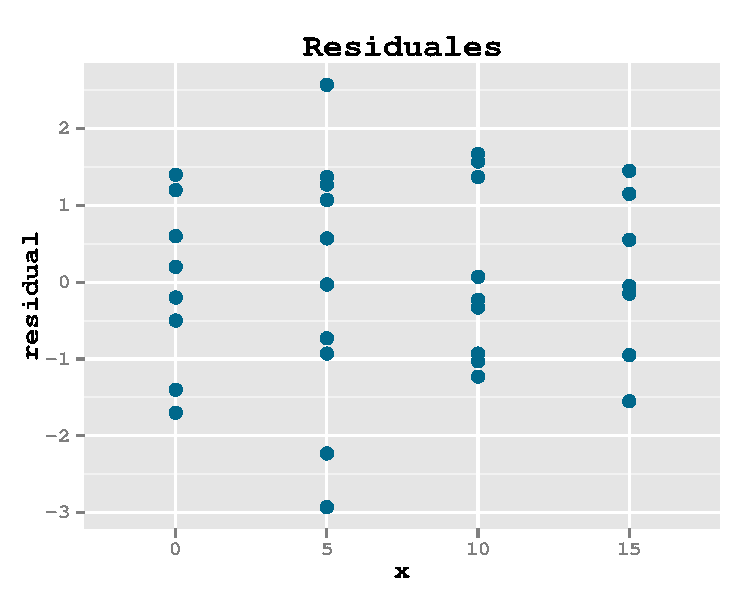
\includegraphics[width=\maxwidth]{figure/unnamed-chunk-172} 

}



\end{knitrout}

\noindent Vemos como siendo estrictos, parece tener colas pesadas la distribución muestral comparadas con la de una normal, y en el caso de los residuales el tratamiento control parece tener una varianza mayor a los demás tratamientos. Ahora veamos las pruebas.

\begin{knitrout}
\definecolor{shadecolor}{rgb}{0.969, 0.969, 0.969}\color{fgcolor}\begin{kframe}
\begin{alltt}
\hlcom{#Prueba de normalidad Anderson-Darling}
\hlkwd{ad.test}\hlstd{(pecesMod}\hlopt{$}\hlstd{res)}
\end{alltt}
\begin{verbatim}
## 
## 	Anderson-Darling normality test
## 
## data:  pecesMod$res
## A = 0.318, p-value = 0.5241
\end{verbatim}
\begin{alltt}
\hlcom{#Prueba de bartlett}
\hlkwd{bartlett.test}\hlstd{(pecesMod}\hlopt{$}\hlstd{res, peces}\hlopt{$}\hlstd{trat)}
\end{alltt}
\begin{verbatim}
## 
## 	Bartlett test of homogeneity of variances
## 
## data:  pecesMod$res and peces$trat
## Bartlett's K-squared = 3.367, df = 3, p-value = 0.3384
\end{verbatim}
\end{kframe}
\end{knitrout}

\noindent Entonces bajo la hipótesis nula de normalidad de los residuales no tenemos evidencia para rechazarla a un nivel de significancia del $5\%$ ($p-value = 0.5241 > 0.05$), análogamente bajo la hipóteis nula de homocedasticidad no tenemos evidencia para rechazar a un nivel de significancia del $5\%$ ($p-value = 0.3384 > 0.05$)

\newpage
\textbf{Problema 6}
Un estudio veterinario busca determinar si el sexo tiene efecto en el peso de los perros, para este estudio se cuenta con lote de 20 perros schnauzer adultos con los siguientes datos:


Se pide que:

\begin{itemize}
  \item Elabore el modelo de diseño de experimentos correspondiente, haciendo explicítos los elementos que lo componen (variable respuesta, factores, supuestos, unidad experimental, ..., etc.)
\end{item}

\noindent\emph{Variable respuesta}: Peso del perro (kg)\\
\emph{Unidad experimental}: Perro\\
\emph{Factor(es)}: Sexo del perro\\
\emph{Niveles}: 2 niveles (macho o hembra)\\

\noindent Además debemos suponer que los perros son homogeneos, lo cuál involucra que se consideren similares en el rango de edad, dieta, raza, y que esten sanos. También contemplar un muestreo adecuado para considerar representatividad.

\begin{itemize}
  \item Elabore la gráfica de tratamientos-peso, analícela y determine si existe evidencia visual para determinar la igualda de los tratamientos
\end{item}

\begin{knitrout}
\definecolor{shadecolor}{rgb}{0.969, 0.969, 0.969}\color{fgcolor}

{\centering 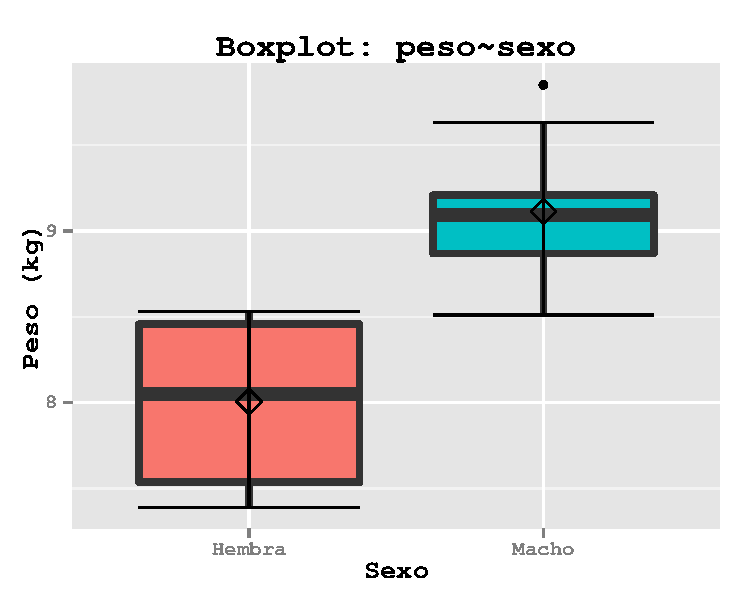
\includegraphics[width=\maxwidth]{figure/unnamed-chunk-19} 

}



\end{knitrout}

Apartir del gráfico podemos ver que en promedio el peso de los perros machos es mayor al de las hembras, además de tener un variabilidad mayor el peso de los machos.

\begin{itemize}
  \item Construya la tabla ANOVA, analícela y concluya ($\alpha = 0.05$)
\end{itemize}

\begin{knitrout}
\definecolor{shadecolor}{rgb}{0.969, 0.969, 0.969}\color{fgcolor}\begin{kframe}
\begin{alltt}
\hlkwd{myANDEVA}\hlstd{(}\hlkwc{n} \hlstd{=} \hlnum{20}\hlstd{,} \hlkwc{t} \hlstd{=} \hlnum{2}\hlstd{,} \hlkwc{data} \hlstd{= perros,} \hlkwc{value} \hlstd{=} \hlstr{"peso"}\hlstd{,} \hlkwc{factor} \hlstd{=} \hlstr{"sexo"}\hlstd{)}
\end{alltt}
\begin{verbatim}
##              g.l. S.S. C.M.     F p-value
## Tratamientos    1 6.12 6.12 29.83       0
## Error          18 3.69 0.21              
## Total          19 9.82
\end{verbatim}
\begin{alltt}
\hlcom{# O ajustando el modelo}
\hlstd{perrosMod} \hlkwb{<-} \hlkwd{lm}\hlstd{(peso} \hlopt{~} \hlstd{sexo,} \hlkwc{data} \hlstd{= perros)}
\hlkwd{anova}\hlstd{(perrosMod)}
\end{alltt}
\begin{verbatim}
## Analysis of Variance Table
## 
## Response: peso
##           Df Sum Sq Mean Sq F value  Pr(>F)    
## sexo       1   6.12    6.12    29.8 3.5e-05 ***
## Residuals 18   3.69    0.21                    
## ---
## Signif. codes:  0 '***' 0.001 '**' 0.01 '*' 0.05 '.' 0.1 ' ' 1
\end{verbatim}
\end{kframe}
\end{knitrout}

\noindent Entonces con una significancia del $5\%$ rechazamos la hipótesis nula de igualda de medias ($p-value = 3.5e-05 < 0.05$). Lo cuál reafirma lo que observamos con el boxplot.

\begin{itemize}
  \item Determine qué tratamientos tienen efectos estadísticamente iguales
\end{itemize}

\noindent Dado que en este caso sólo tenemos dos tratamientos y lo anterior, podemos decir que con una significancia del $5\%$ el promedio del peso de los machos es mayor al de las hembras.\\

\begin{itemize}
  \item Construya las gráficas de los residuos necesarias para verificar los supuestos de homocedasticidad y normalidad. Utilice la prueba de Bartlett para verificar el supuesto de homogeneidad de varianzas 
\end{itemize}

\begin{knitrout}
\definecolor{shadecolor}{rgb}{0.969, 0.969, 0.969}\color{fgcolor}

{\centering 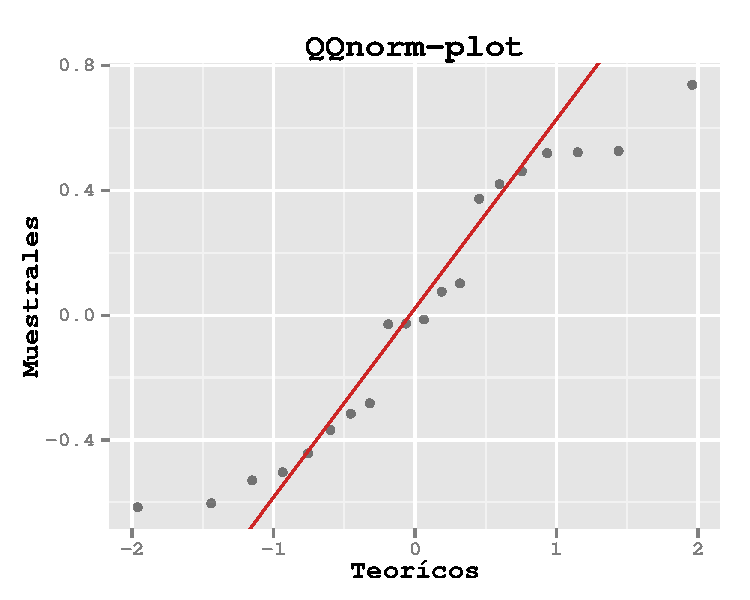
\includegraphics[width=\maxwidth]{figure/unnamed-chunk-211} 

}




{\centering 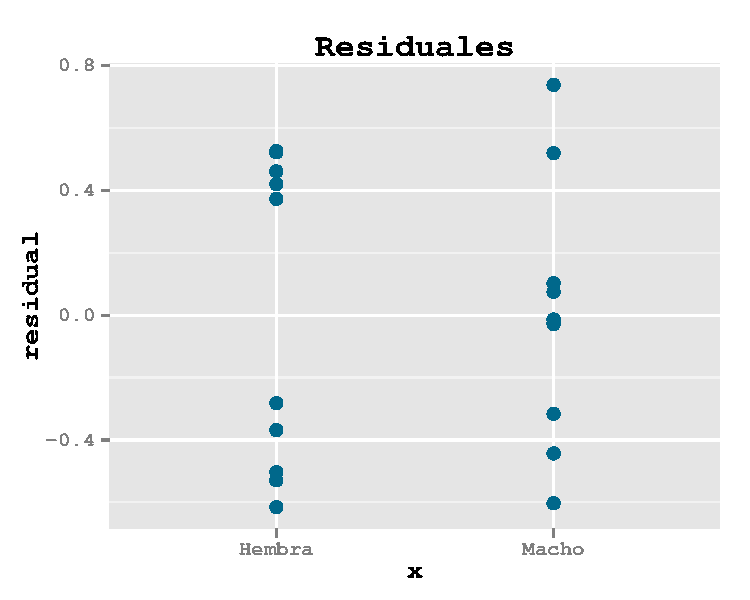
\includegraphics[width=\maxwidth]{figure/unnamed-chunk-212} 

}



\end{knitrout}

\noindent Vemos como siendo estrictos, parece que en las colas la distribución muestral no se parece a una normal, y en el caso de los residuales el peso en los machos parece tener una varianza similar al de las hembras. Ahora veamos las pruebas.

\begin{knitrout}
\definecolor{shadecolor}{rgb}{0.969, 0.969, 0.969}\color{fgcolor}\begin{kframe}
\begin{alltt}
\hlcom{#Prueba de normalidad Anderson-Darling}
\hlkwd{ad.test}\hlstd{(perrosMod}\hlopt{$}\hlstd{res)}
\end{alltt}
\begin{verbatim}
## 
## 	Anderson-Darling normality test
## 
## data:  perrosMod$res
## A = 0.5624, p-value = 0.1265
\end{verbatim}
\begin{alltt}
\hlcom{#Prueba de bartlett}
\hlkwd{bartlett.test}\hlstd{(perrosMod}\hlopt{$}\hlstd{res, perros}\hlopt{$}\hlstd{sexo)}
\end{alltt}
\begin{verbatim}
## 
## 	Bartlett test of homogeneity of variances
## 
## data:  perrosMod$res and perros$sexo
## Bartlett's K-squared = 0.3224, df = 1, p-value = 0.5702
\end{verbatim}
\end{kframe}
\end{knitrout}

\noindent Entonces bajo la hipótesis nula de normalidad de los residuales no tenemos evidencia para rechazarla a un nivel de significancia del $5\%$ ($p-value =  0.1265 > 0.05$), análogamente bajo la hipóteis nula de homocedasticidad no tenemos evidencia para rechazar a un nivel de significancia del $5\%$ ($p-value =  0.5702 > 0.05$)

\newpage
\textbf{Problema 7}
Utilizando los datos \emph{KenyaFinches} contenidos en la librería \emph{abd} del programa R, determine si la subespecie de los pinzones es un factor determinante en la longitud del pico de los pinzones.

Se pide que:

\begin{itemize}
  \item Elabore el modelo de diseño de experimentos correspondiente, haciendo explicítos los elementos que lo componen (variable respuesta, factores, supuestos, unidad experimental, ..., etc.)
\end{item}

\begin{knitrout}
\definecolor{shadecolor}{rgb}{0.969, 0.969, 0.969}\color{fgcolor}\begin{kframe}
\begin{alltt}
\hlkwd{str}\hlstd{(KenyaFinches)}
\end{alltt}
\begin{verbatim}
## 'data.frame':	45 obs. of  3 variables:
##  $ species    : Factor w/ 3 levels "CRU.WAXB","CUTTHROA",..: 3 3 3 3 3 3 3 3 3 3 ...
##  $ mass       : int  40 43 37 38 43 33 35 37 36 42 ...
##  $ beak.length: num  10.6 10.8 10.9 11.3 10.9 10.1 10.7 10.7 10.9 11.4 ...
\end{verbatim}
\begin{alltt}
\hlcom{# Veamos una mestra de la base}
\hlkwd{sample}\hlstd{(KenyaFinches,} \hlnum{6}\hlstd{)[,} \hlopt{-}\hlnum{4}\hlstd{]}
\end{alltt}
\begin{verbatim}
##     species mass beak.length
## 30 CRU.WAXB    8         7.1
## 18 CRU.WAXB    8         7.2
## 24 CRU.WAXB    6         6.9
## 9  WB.SPARW   36        10.9
## 41 CUTTHROA   17         8.7
## 14 WB.SPARW   37        10.0
\end{verbatim}
\begin{alltt}
\hlcom{# Observamos el número de observaciones por pinzón}
\hlkwd{table}\hlstd{(KenyaFinches}\hlopt{$}\hlstd{species)}
\end{alltt}
\begin{verbatim}
## 
## CRU.WAXB CUTTHROA WB.SPARW 
##       17       12       16
\end{verbatim}
\end{kframe}
\end{knitrout}

\noindent Esta base de datos considera información sobre el peso y longitud del pico de tres especies de pinzones. Y porn lo anterior vemos que se trata de un diseño desbalanceado.

\noindent\emph{Variable respuesta}: Peso y longitud del pico.
\emph{Unidad experimental}: Pinzón
\emph{Factor(es)}: 3 especie del pinzón (denotadas por: CRU.WAXB, CUTTHROA y WB.SPARW)


\begin{itemize}
  \item Elabore la gráfica de tratamientos-longitud, analícela y determine si existe evidencia visual para determinar la igualda de los tratamientos
\end{item}

\begin{knitrout}
\definecolor{shadecolor}{rgb}{0.969, 0.969, 0.969}\color{fgcolor}

{\centering 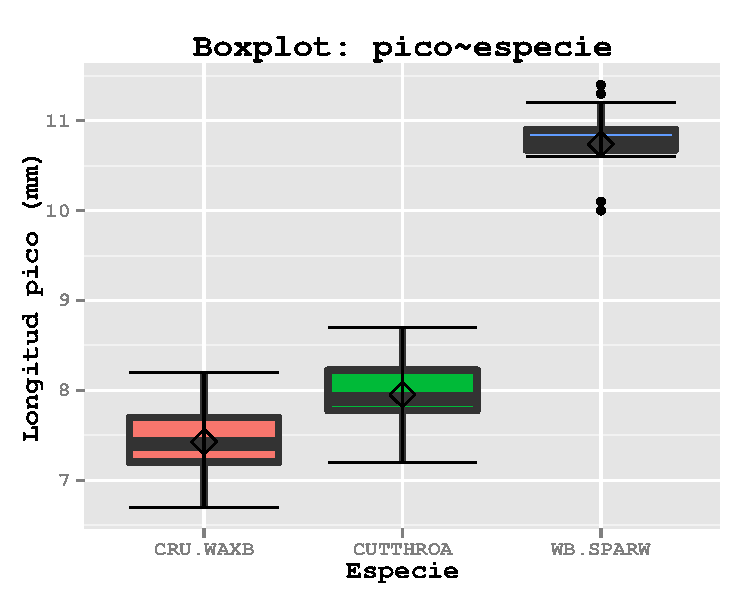
\includegraphics[width=\maxwidth]{figure/unnamed-chunk-24} 

}



\end{knitrout}

\noindent Por el boxplot podemos observar que la longitud del pico de las especies CRU.WAXB y CUTTHROA son algo similares entre si pero difieren de la especie WB.SPARW.

\begin{itemize}
  \item Construya la tabla ANOVA, analícela y concluya ($\alpha = 0.05$)
\end{itemize}

\begin{knitrout}
\definecolor{shadecolor}{rgb}{0.969, 0.969, 0.969}\color{fgcolor}\begin{kframe}
\begin{alltt}
\hlkwd{myANDEVA}\hlstd{(}\hlkwc{n} \hlstd{=} \hlnum{45}\hlstd{,} \hlkwc{t} \hlstd{=} \hlnum{3}\hlstd{,} \hlkwc{data} \hlstd{= KenyaFinches,}
         \hlkwc{value} \hlstd{=} \hlstr{"beak.length"}\hlstd{,} \hlkwc{factor} \hlstd{=} \hlstr{"species"}\hlstd{)}
\end{alltt}
\begin{verbatim}
##              g.l.   S.S.  C.M.     F p-value
## Tratamientos    2 100.53 50.26 303.2       0
## Error          42   6.96  0.17              
## Total          44 107.49
\end{verbatim}
\begin{alltt}
\hlcom{# O ajustando el modelo}
\hlstd{pinzonMod} \hlkwb{<-} \hlkwd{lm}\hlstd{(beak.length} \hlopt{~} \hlstd{species,} \hlkwc{data} \hlstd{= KenyaFinches)}
\hlkwd{anova}\hlstd{(pinzonMod)}
\end{alltt}
\begin{verbatim}
## Analysis of Variance Table
## 
## Response: beak.length
##           Df Sum Sq Mean Sq F value Pr(>F)    
## species    2    100    50.3     303 <2e-16 ***
## Residuals 42      7     0.2                   
## ---
## Signif. codes:  0 '***' 0.001 '**' 0.01 '*' 0.05 '.' 0.1 ' ' 1
\end{verbatim}
\end{kframe}
\end{knitrout}

\noindent Por lo que con una significancia del $5\%$ tenemos evidencia para rechaza la hipótesis nula de igualdad de medias ($p-value = 2.2e-16 < 0.05$), es decir que al menos una de las especies difiere en el promedio de la longitud de su pico con respecto a las otras.

\begin{itemize}
  \item Determine qué tratamientos tienen efectos estadísticamente iguales
\end{itemize}

\noindent Para esto usaremos la prueba de Tukey:

\begin{knitrout}
\definecolor{shadecolor}{rgb}{0.969, 0.969, 0.969}\color{fgcolor}\begin{kframe}
\begin{alltt}
\hlcom{# Prueba de Tukey}
\hlstd{tukey} \hlkwb{<-} \hlkwd{TukeyHSD}\hlstd{(}\hlkwd{aov}\hlstd{(pinzonMod),} \hlkwc{conf.level} \hlstd{=} \hlnum{0.95}\hlstd{); tukey}
\end{alltt}
\begin{verbatim}
##   Tukey multiple comparisons of means
##     95% family-wise confidence level
## 
## Fit: aov(formula = pinzonMod)
## 
## $species
##                     diff    lwr    upr  p adj
## CUTTHROA-CRU.WAXB 0.5206 0.1476 0.8936 0.0043
## WB.SPARW-CRU.WAXB 3.3081 2.9635 3.6526 0.0000
## WB.SPARW-CUTTHROA 2.7875 2.4097 3.1653 0.0000
\end{verbatim}
\end{kframe}
\end{knitrout}

\noindent Por lo qué lo que observamos diferencias significativas ($\alpha = 0.05$) entre las distintas especies. Gráficamente podemos ver los intervalos de confianza.

\begin{knitrout}
\definecolor{shadecolor}{rgb}{0.969, 0.969, 0.969}\color{fgcolor}

{\centering 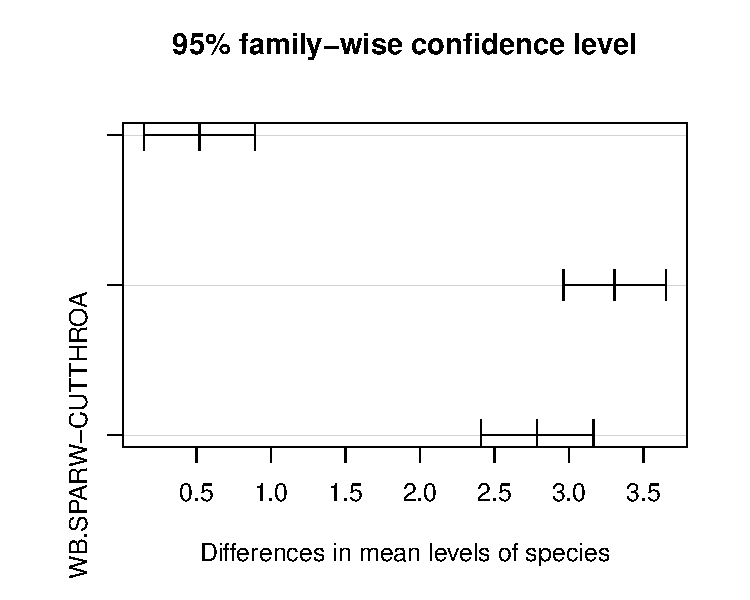
\includegraphics[width=\maxwidth]{figure/unnamed-chunk-27} 

}



\end{knitrout}

\begin{itemize}
  \item Construya las gráficas de los residuos necesarias para verificar los supuestos de homocedasticidad y normalidad. Utilice la prueba de Bartlett para verificar el supuesto de homogeneidad de varianzas 
\end{itemize}

\begin{knitrout}
\definecolor{shadecolor}{rgb}{0.969, 0.969, 0.969}\color{fgcolor}

{\centering 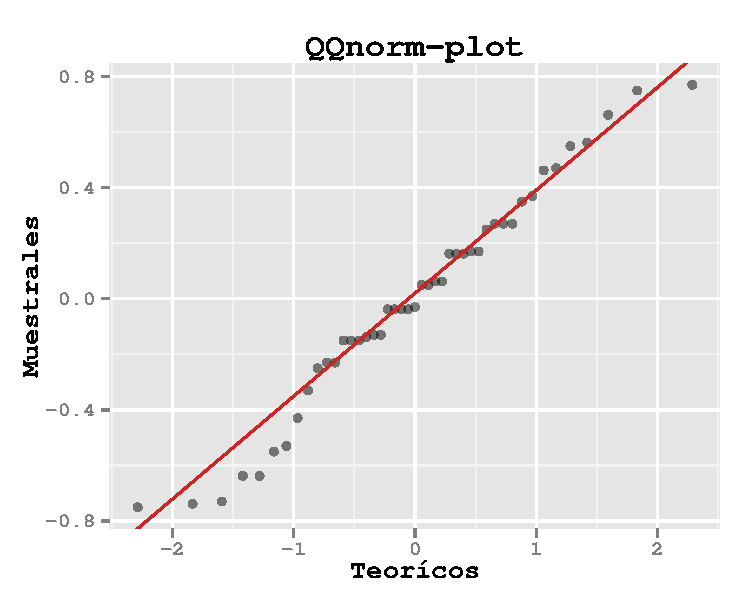
\includegraphics[width=\maxwidth]{figure/unnamed-chunk-281} 

}




{\centering 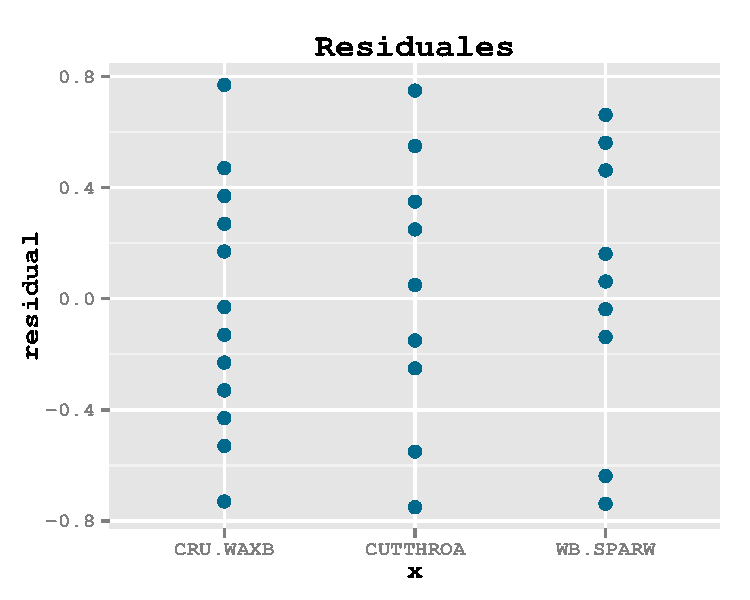
\includegraphics[width=\maxwidth]{figure/unnamed-chunk-282} 

}



\end{knitrout}

\noindent Vemos que parece que no se debe rechazar la hipótesis de normalidad de los datos, y en el caso de los residuales tampoco parece haber motivos para rechazar la hipótesis de homocedasticidad. Ahora veamos las pruebas.

\begin{knitrout}
\definecolor{shadecolor}{rgb}{0.969, 0.969, 0.969}\color{fgcolor}\begin{kframe}
\begin{alltt}
\hlcom{#Prueba de normalidad Anderson-Darling}
\hlkwd{ad.test}\hlstd{(pinzonMod}\hlopt{$}\hlstd{res)}
\end{alltt}
\begin{verbatim}
## 
## 	Anderson-Darling normality test
## 
## data:  pinzonMod$res
## A = 0.2985, p-value = 0.5719
\end{verbatim}
\begin{alltt}
\hlcom{#Prueba de bartlett}
\hlkwd{bartlett.test}\hlstd{(pinzonMod}\hlopt{$}\hlstd{res, KenyaFinches}\hlopt{$}\hlstd{species)}
\end{alltt}
\begin{verbatim}
## 
## 	Bartlett test of homogeneity of variances
## 
## data:  pinzonMod$res and KenyaFinches$species
## Bartlett's K-squared = 0.115, df = 2, p-value = 0.9441
\end{verbatim}
\end{kframe}
\end{knitrout}

\noindent Entonces bajo la hipótesis nula de normalidad de los residuales no tenemos evidencia para rechazarla a un nivel de significancia del $5\%$ ($p-value = 0.5719 > 0.05$), análogamente bajo la hipóteis nula de homocedasticidad no tenemos evidencia para rechazar a un nivel de significancia del $5\%$ ($p-value = 0.9441 > 0.05$)

\end{document}
